\section{Summary of Findings} \label{section:summary_of_findings}

% ---------- %

This study evaluated whether machine-learned interatomic potentials (MLPs), specifically the MACE framework, can
replicate DFT-derived rankings of interface stability across group-IV systems, including carbon (C), silicon (Si),
germanium (Ge), and tin (Sn).

The investigation involved automated structure generation via ARTEMIS, energy evaluation using both DFT and MLP on
unrelaxed geometries, and statistical analysis of ranking agreement using Spearman $\rho$, Kendall $\tau$, and Top-N
overlap.

% ---------- %

Rather than comparing relaxed geometries, all interfaces were evaluated in their unrelaxed form to isolate differences
in energy prediction.

This enabled a fair, geometry-matched comparison of MLP vs DFT across a large dataset, while identifying how system
composition and stacking geometry impact rank preservation.

% ---------- %

Agreement between MLP and DFT was found to be strongly system-dependent.

MLPs performed exceptionally well for Ge and Sn systems, achieving high rank correlation ($\rho > 0.97$) and Top-10
overlap ($\sim$8/10) with DFT rankings.

For Si-based systems, especially those where Si appeared in the lower slab, rank correlation deteriorated significantly
(e.g. $\rho \approx 0.62$), suggesting sensitivity to stacking order and geometric artefacts.

These failures appeared systematic rather than statistical, highlighting specific challenges for MLPs in strained or
under-coordinated bonding environments.

% ---------- %

% todo: check if i want to keep the figure below
%\begin{figure}[h]
%    \centering
%    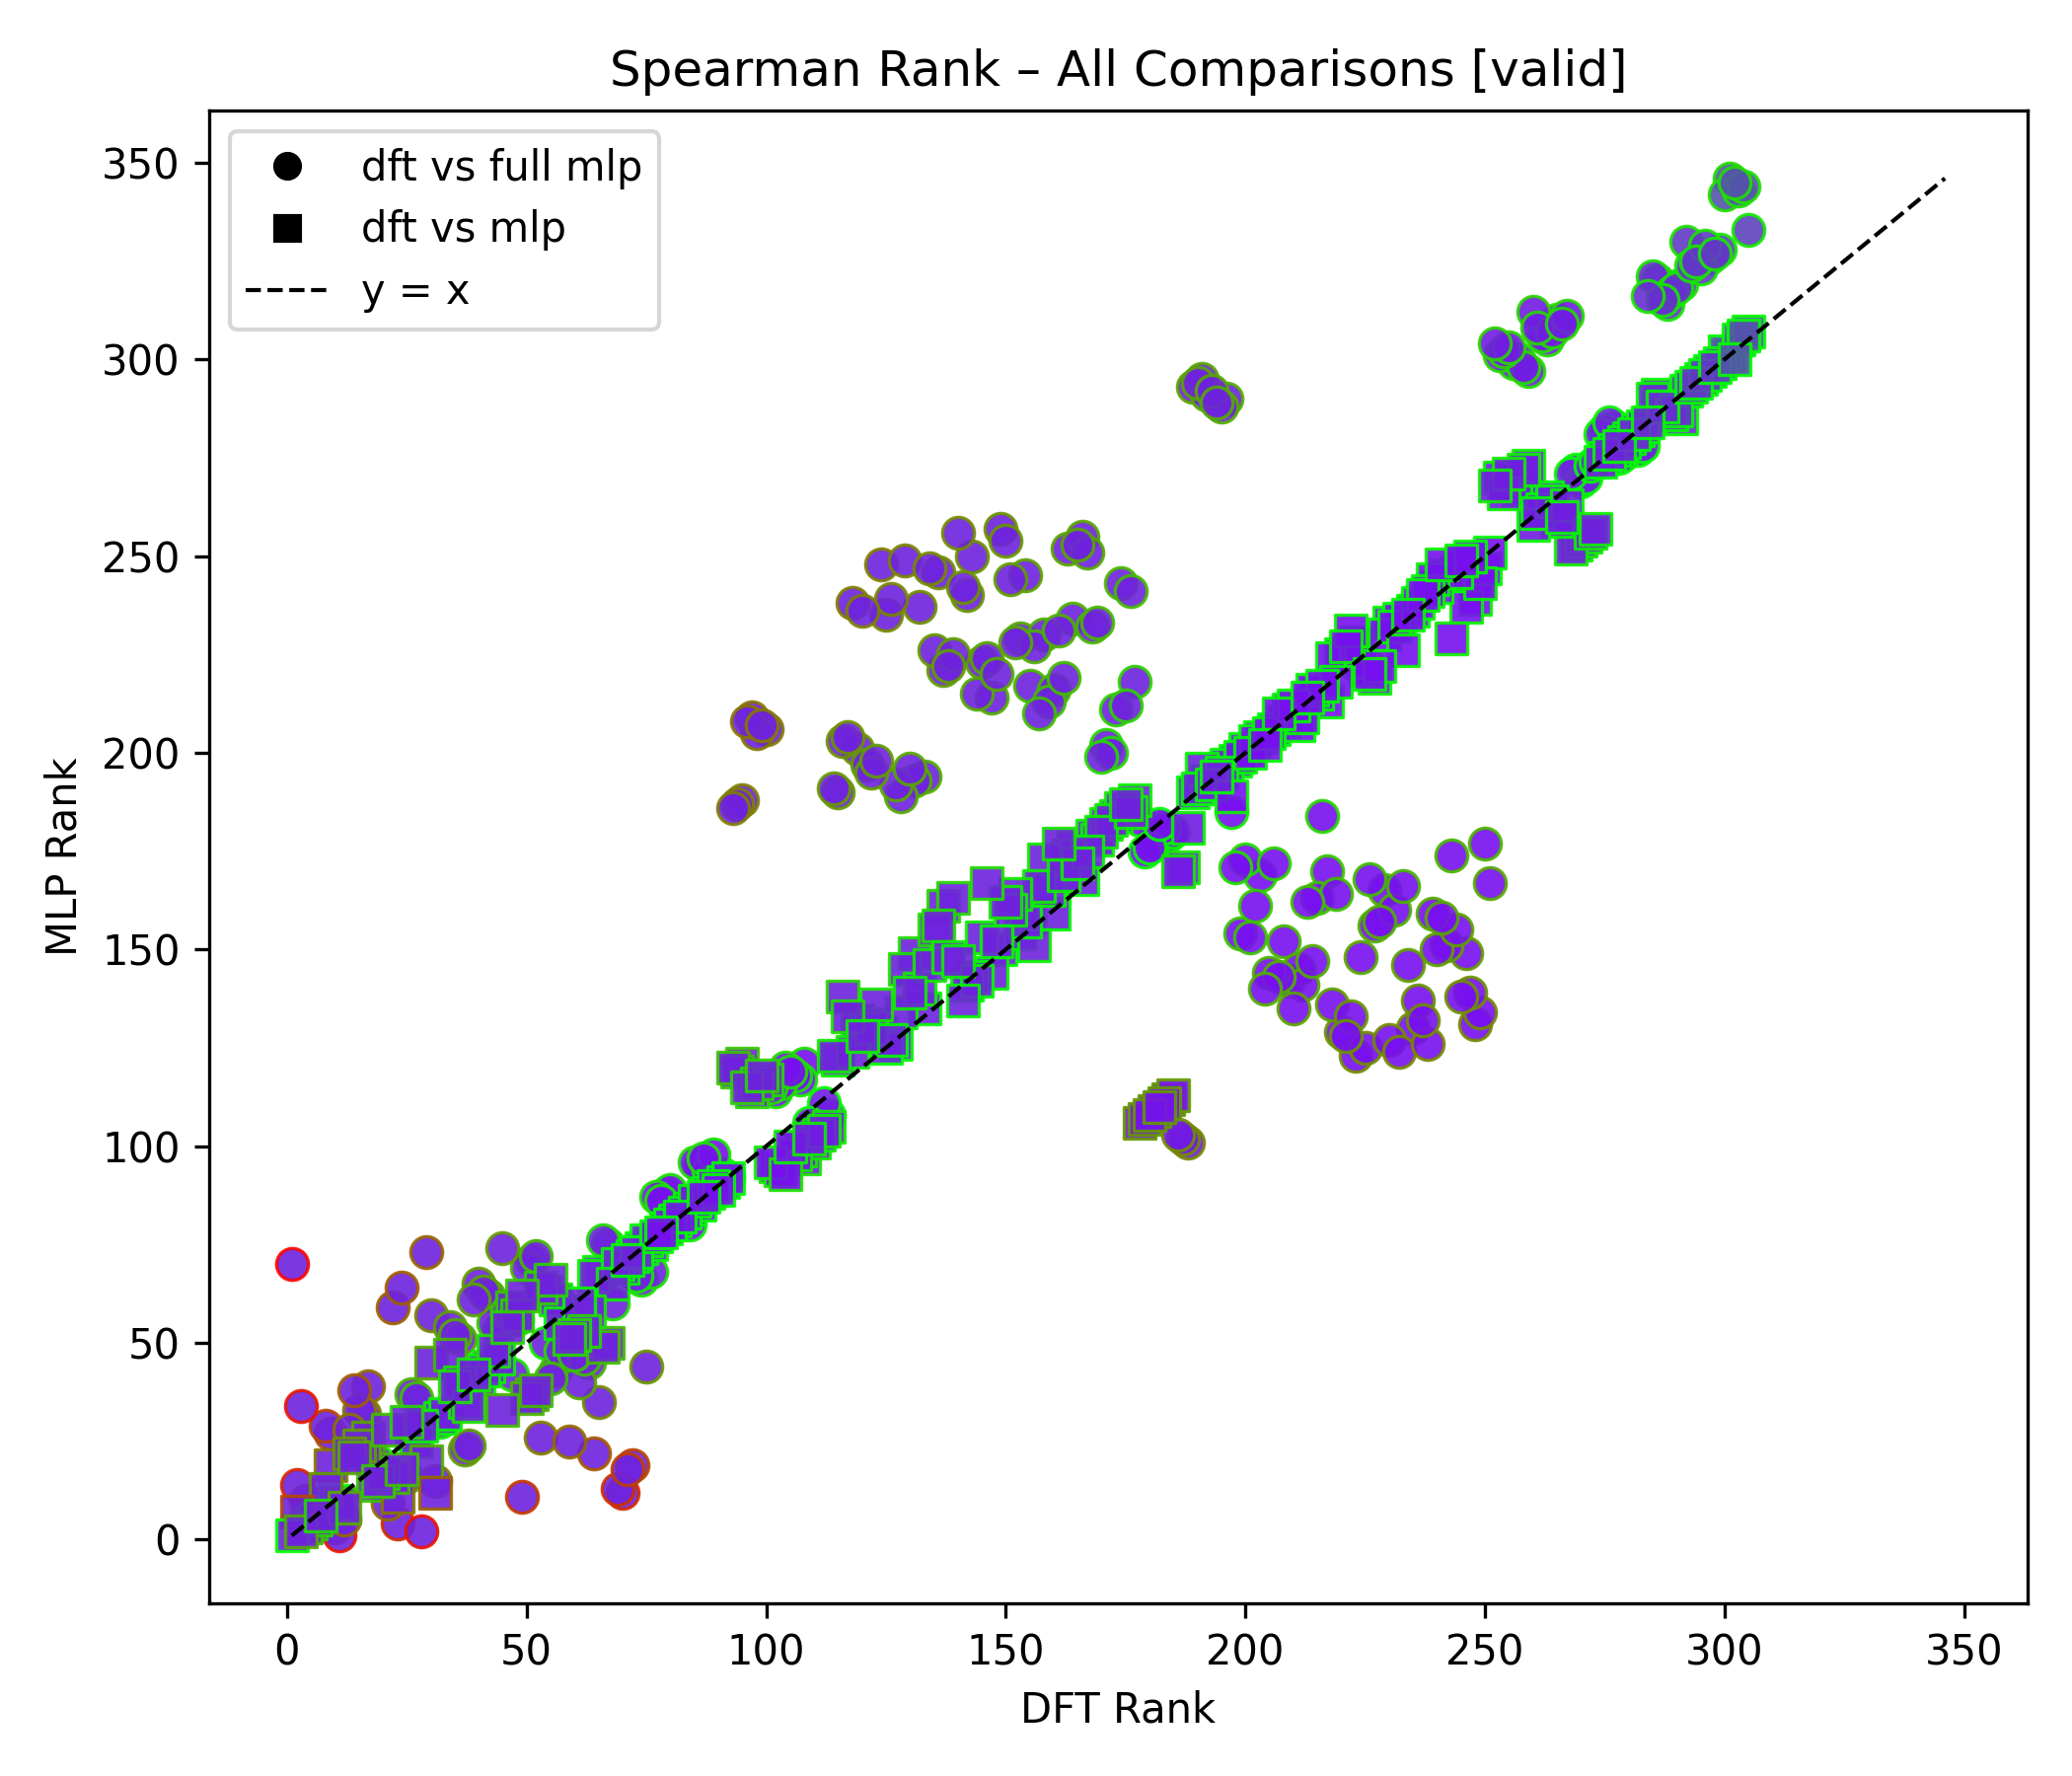
\includegraphics[width=0.7\textwidth]{analysis/plots/results_lower_Si_spearman_all_comparisons_valid.png}
%    \caption{Spearman rank correlation for Si interfaces, showing weak rank preservation in lower-Si systems due to geometric artefacts and interfacial strain.}
%\end{figure}

% ---------- %

Carbon results were geometry-dependent: only three valid C|Si structures with carbon in the lower slab were obtained,
and these yielded unreliable results ($\rho = -0.5$), leading to their exclusion from analysis.

However, when carbon appeared in the upper slab (C|X), rank correlation was excellent ($\rho = 0.95$), and MAE dropped
below 1 eV. Silicon systems, especially Si|Ge, consistently showed weaker performance, while Ge|Si demonstrated improved
alignment.

Germanium and tin systems showed robust rank preservation and strong Top-N screening performance across the board.

% ---------- %

% todo: check if i want to keep the figure below
%\begin{table}[h]
%    \centering
%    \caption{Performance metrics for Si interfaces (Si in upper slab) from \texttt{analysis/stats_upper_Si.csv}. Lower-slab Si configurations exhibited even poorer rank correlation (not shown), highlighting geometry sensitivity.}
%    \begin{tabular}{lcccccc}
%        Comparison & Spearman & Kendall & RMSE & MAE & Top-10 Overlap \\
%        \hline
%        DFT@DFT vs MLP@MLP & 0.46 & 0.31 & 7.48 & 3.36 & 3 \\
%    \end{tabular}
%\end{table}

% ---------- %

Although direct MLP-on-DFT-relaxed structure evaluations (MLP@DFT) were not included due to computational cost, the
study revealed that relaxation, evaluation consistency (e.g. MLP@MLP vs DFT@DFT) influences error, and future
cross-evaluation may further clarify error sources.

% ---------- %

% todo: [placeholder, for: future figure showing relaxation-evaluation matrix comparisons]

% ---------- %

\subsection{Interface Rank Preservation} \label{section:interface_rank_preservation}

% ---------- %

While absolute energy errors between MLP and DFT were large (e.g. RMSE ≈ 189 eV), they were secondary to the study's
goal of rank preservation.

In this context, MLPs effectively captured the energetic hierarchy of Ge and Sn interfaces.

% ---------- %

\begin{figure}[h]
    \centering
    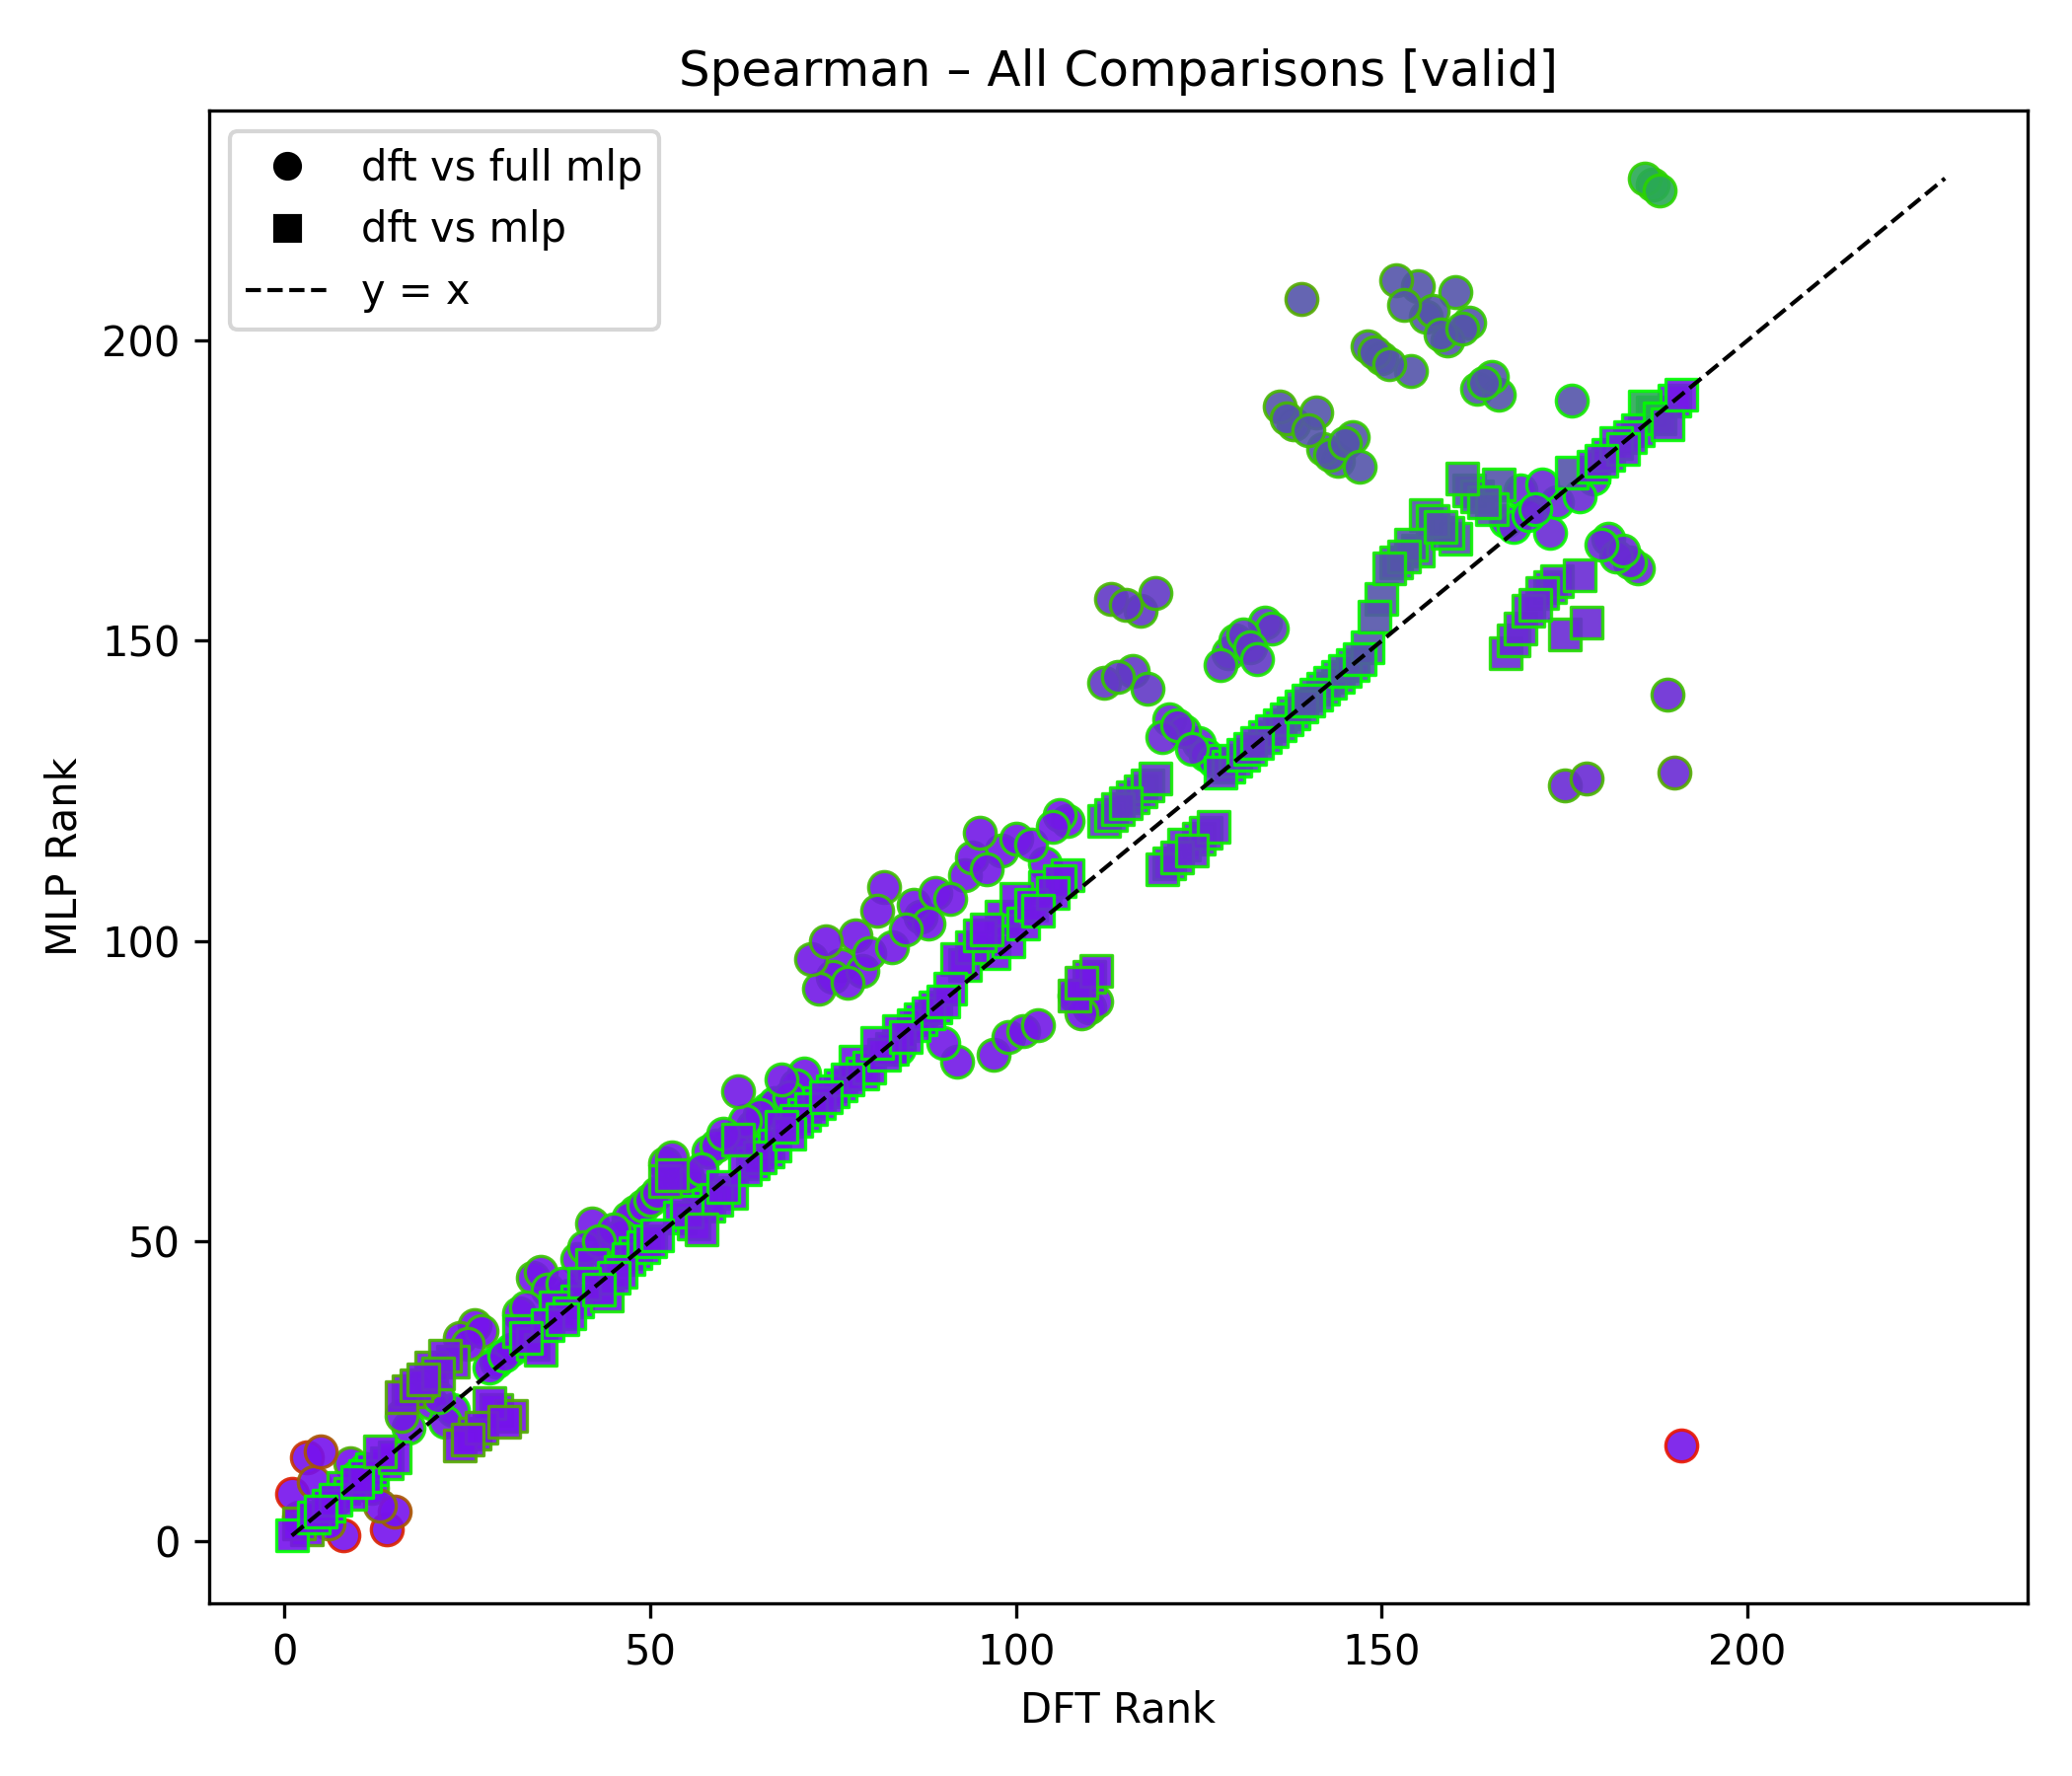
\includegraphics[width=0.7\textwidth]{analysis/plots/results_lower_Ge_spearman_all_comparisons_valid.png}
    \caption{Spearman correlation for Ge interfaces.}
\end{figure}

% ---------- %

Top-N overlap and rank correlation metrics confirmed that MLPs are useful for screening favourable structures,
especially in Ge and Sn systems.

Even when absolute energy values deviated significantly, the identity of the top-ranked configurations was largely
preserved, with 8 out of 10 matches in many systems.

This supports the use of MLPs like MACE in high-throughput pre-screening pipelines to prioritise candidates for costly
DFT relaxation.

% ---------- %

\begin{figure}[h]
    \centering
    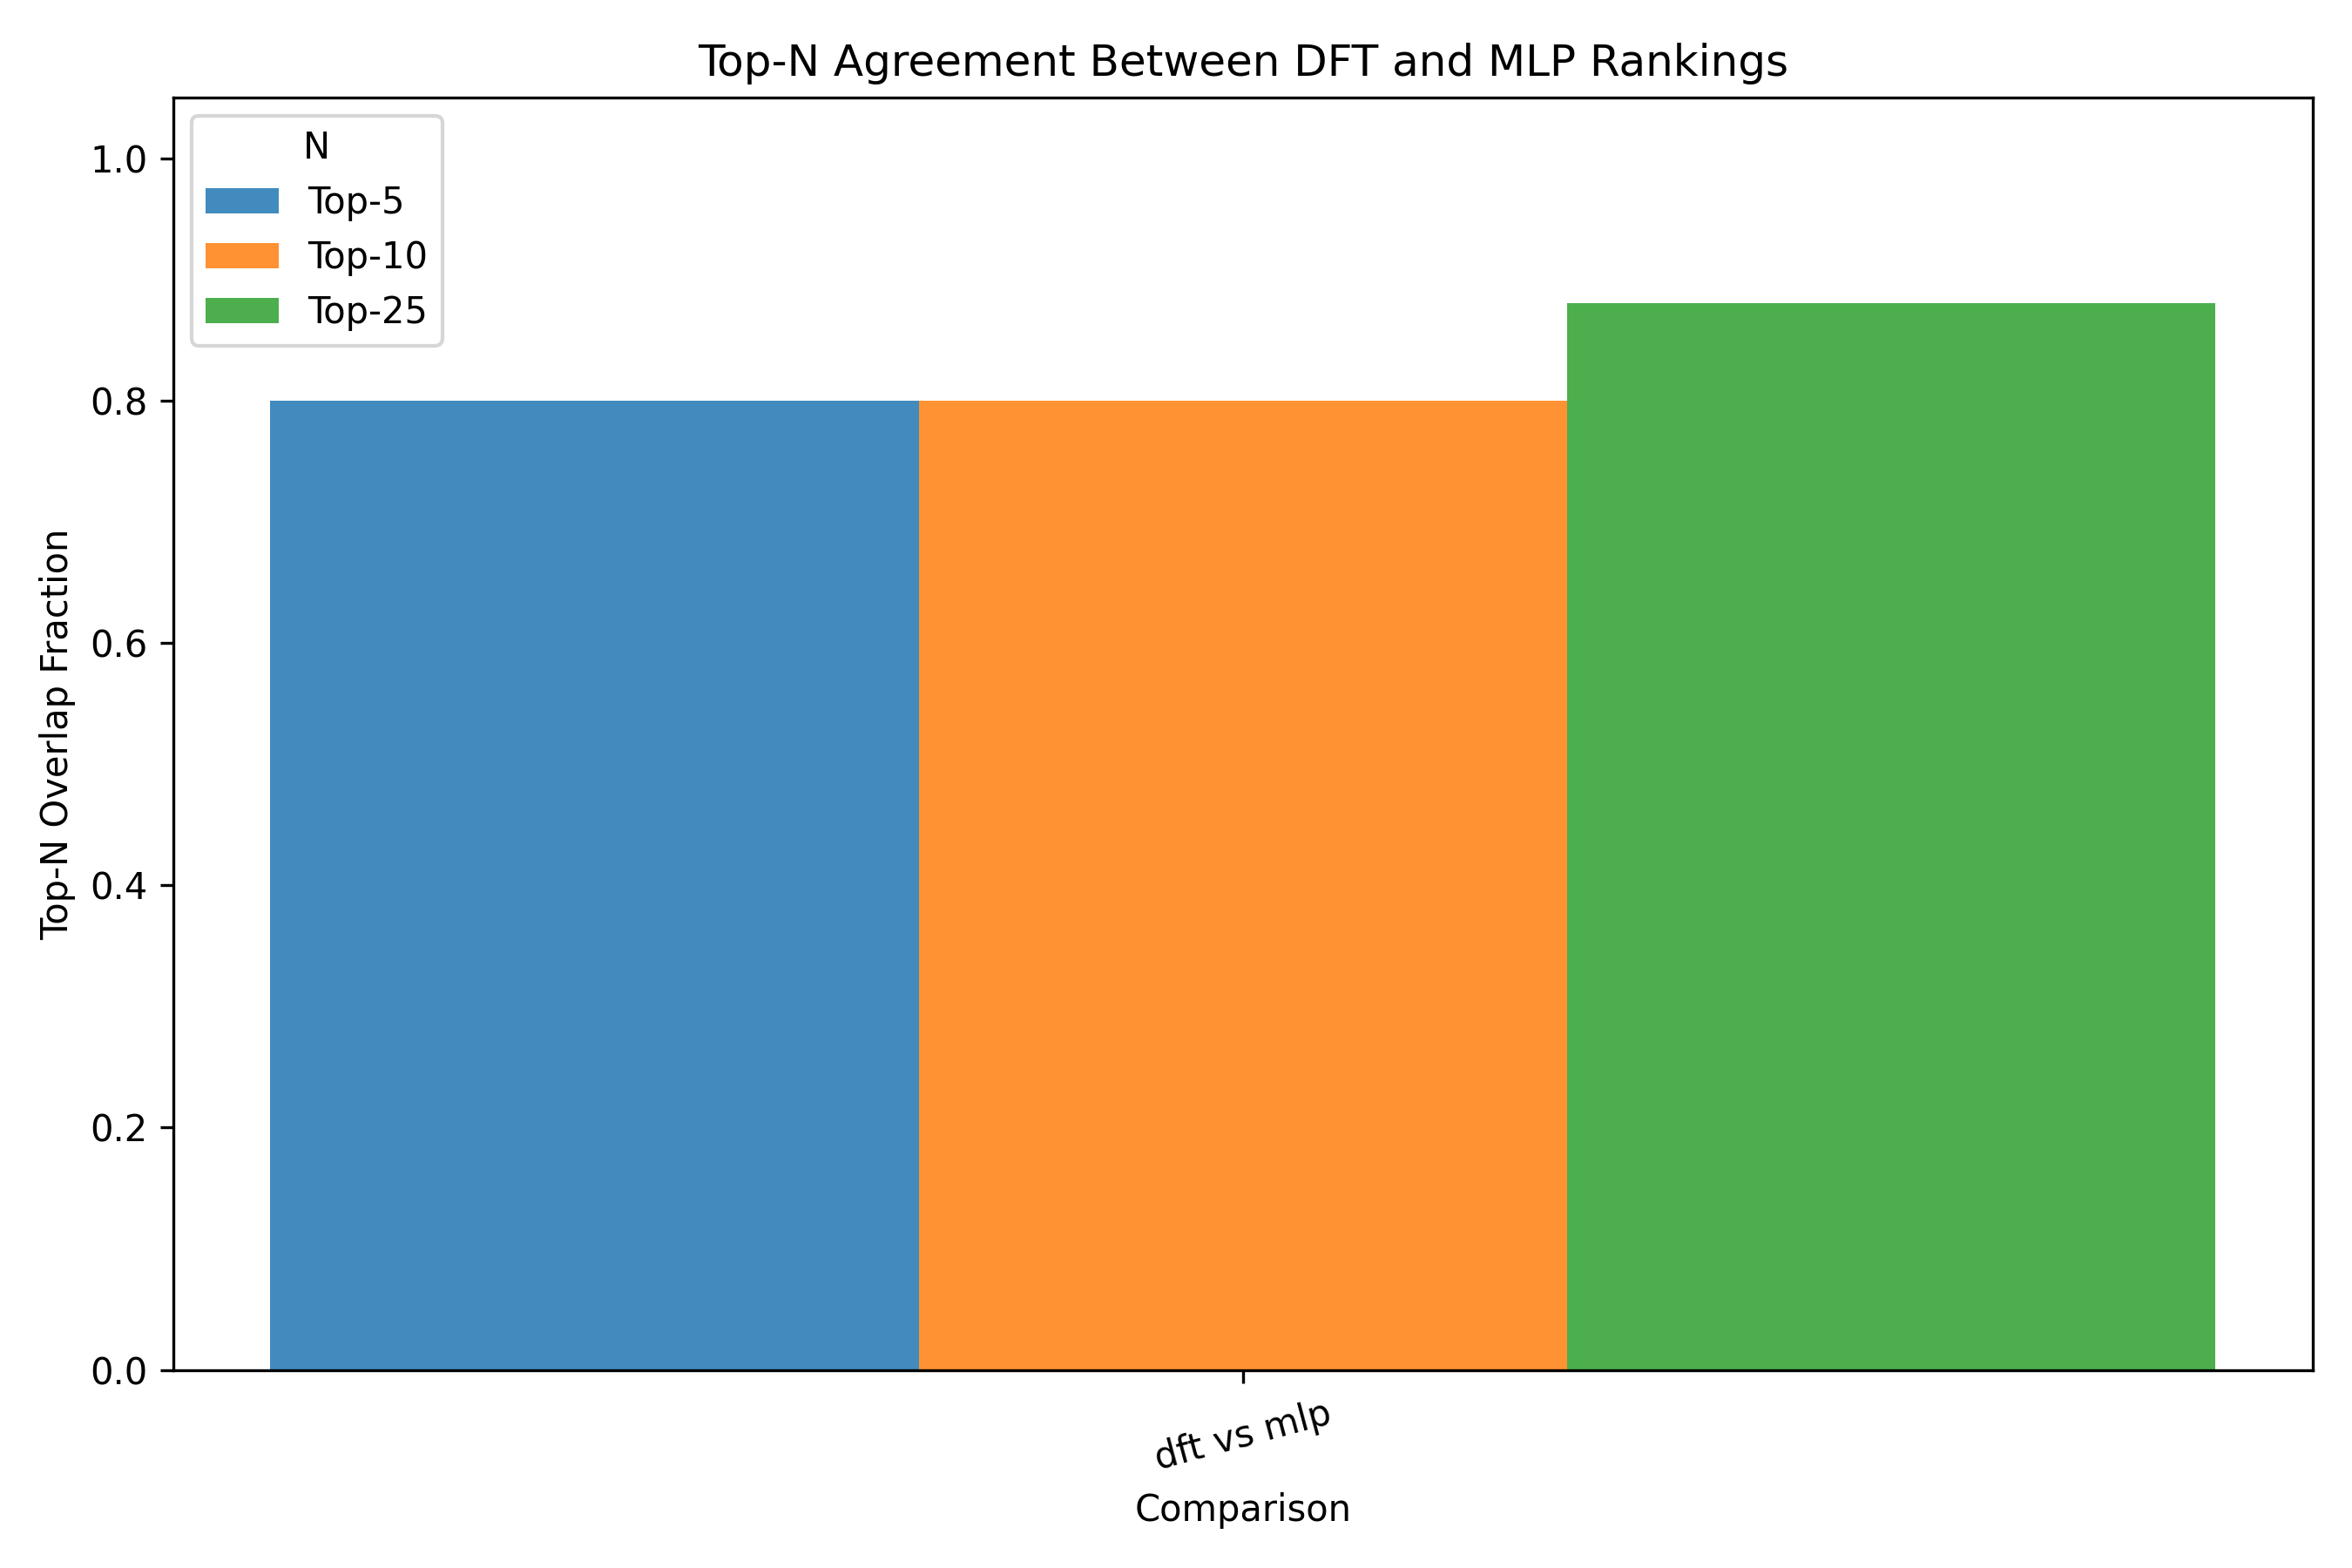
\includegraphics[width=0.7\textwidth]{analysis/plots/results_lower_Si_topn_overlap.png}
    \caption{Top-\textit{N} overlap for Si interfaces.}
\end{figure}

% ---------- %

MLPs offer significant computational speed advantages and can be reliably used for preliminary screening in systems with
well-represented local bonding environments, such as Ge, Sn, and some C|X combinations.

However, their generalisation is limited in strained or covalently dominated systems like Si|X, particularly when poor
coordination or stacking asymmetry is present.

Without targeted retraining or domain-specific corrections, MLP-based predictions in such cases may be misleading.

% ---------- %

% todo: add Equation suggestion: O(n) comparison of DFT vs MLP computational cost per electron.

% ---------- %